% Options for packages loaded elsewhere
\PassOptionsToPackage{unicode}{hyperref}
\PassOptionsToPackage{hyphens}{url}
%
\documentclass[
]{article}
\usepackage{amsmath,amssymb}
\usepackage{iftex}
\ifPDFTeX
  \usepackage[T1]{fontenc}
  \usepackage[utf8]{inputenc}
  \usepackage{textcomp} % provide euro and other symbols
\else % if luatex or xetex
  \usepackage{unicode-math} % this also loads fontspec
  \defaultfontfeatures{Scale=MatchLowercase}
  \defaultfontfeatures[\rmfamily]{Ligatures=TeX,Scale=1}
\fi
\usepackage{lmodern}
\ifPDFTeX\else
  % xetex/luatex font selection
\fi
% Use upquote if available, for straight quotes in verbatim environments
\IfFileExists{upquote.sty}{\usepackage{upquote}}{}
\IfFileExists{microtype.sty}{% use microtype if available
  \usepackage[]{microtype}
  \UseMicrotypeSet[protrusion]{basicmath} % disable protrusion for tt fonts
}{}
\makeatletter
\@ifundefined{KOMAClassName}{% if non-KOMA class
  \IfFileExists{parskip.sty}{%
    \usepackage{parskip}
  }{% else
    \setlength{\parindent}{0pt}
    \setlength{\parskip}{6pt plus 2pt minus 1pt}}
}{% if KOMA class
  \KOMAoptions{parskip=half}}
\makeatother
\usepackage{xcolor}
\usepackage[margin=1in]{geometry}
\usepackage{graphicx}
\makeatletter
\def\maxwidth{\ifdim\Gin@nat@width>\linewidth\linewidth\else\Gin@nat@width\fi}
\def\maxheight{\ifdim\Gin@nat@height>\textheight\textheight\else\Gin@nat@height\fi}
\makeatother
% Scale images if necessary, so that they will not overflow the page
% margins by default, and it is still possible to overwrite the defaults
% using explicit options in \includegraphics[width, height, ...]{}
\setkeys{Gin}{width=\maxwidth,height=\maxheight,keepaspectratio}
% Set default figure placement to htbp
\makeatletter
\def\fps@figure{htbp}
\makeatother
\setlength{\emergencystretch}{3em} % prevent overfull lines
\providecommand{\tightlist}{%
  \setlength{\itemsep}{0pt}\setlength{\parskip}{0pt}}
\setcounter{secnumdepth}{-\maxdimen} % remove section numbering
\ifLuaTeX
  \usepackage{selnolig}  % disable illegal ligatures
\fi
\IfFileExists{bookmark.sty}{\usepackage{bookmark}}{\usepackage{hyperref}}
\IfFileExists{xurl.sty}{\usepackage{xurl}}{} % add URL line breaks if available
\urlstyle{same}
\hypersetup{
  hidelinks,
  pdfcreator={LaTeX via pandoc}}

\author{}
\date{\vspace{-2.5em}}

\begin{document}

\hypertarget{hw-1---cs-625-fall-2023}{%
\section{HW 1 - CS 625, Fall 2023}\label{hw-1---cs-625-fall-2023}}

Eswari Kannipoti\\
Due: September 6, 2023

\hypertarget{git-github}{%
\subsection{Git, GitHub}\label{git-github}}

\emph{What is the URL of the GitHub repo that you created in your
personal account?}

\begin{verbatim}
https://github.com/Eswarikannipoti/HW-1-report/
\end{verbatim}

\emph{In which direction does the `pull' command work (send local
changes to remote OR send remote changes to local)?} The Pull command is
used to send remote changes to local.

\emph{If you have committed a change on your local machine, but do not
see the update on GitHub.com, what step might have you forgotten?} If we
cannot see the update on github we might have forgotten to use the push
command.

\hypertarget{markdown}{%
\subsection{Markdown}\label{markdown}}

\emph{Create a bulleted list with at least 3 items}

Hey, I'm Eswari Kannipoti

\emph{I'm a master's student at ODU}.

\textbf{This is course CR-625}.

I live in 1049 W APR 103.

Google: \href{https://www.google.com/}{google}.

\emph{Write a single paragraph that demonstrates the use of italics,
bold, bold italics, code, and includes a link. The paragraph does not
have to make sense.}

\emph{Create a level 3 heading} \#\#\# FIRST HOME WORK IN MASTERS

\emph{Insert an image of an animal, sized appropriately}
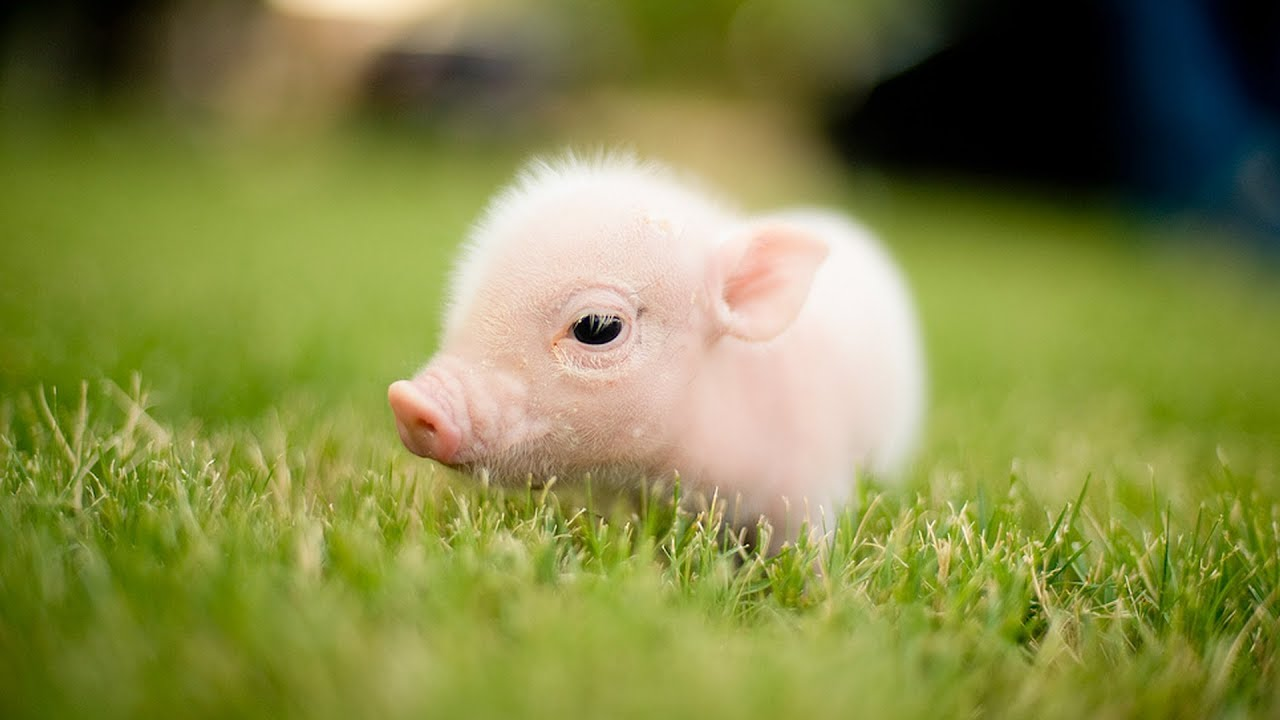
\includegraphics{pig.jpg}

\hypertarget{tableau}{%
\subsection{Tableau}\label{tableau}}

\emph{Insert your the image of your final bar chart here. Reminder, this
should show data from a region other than the South.}
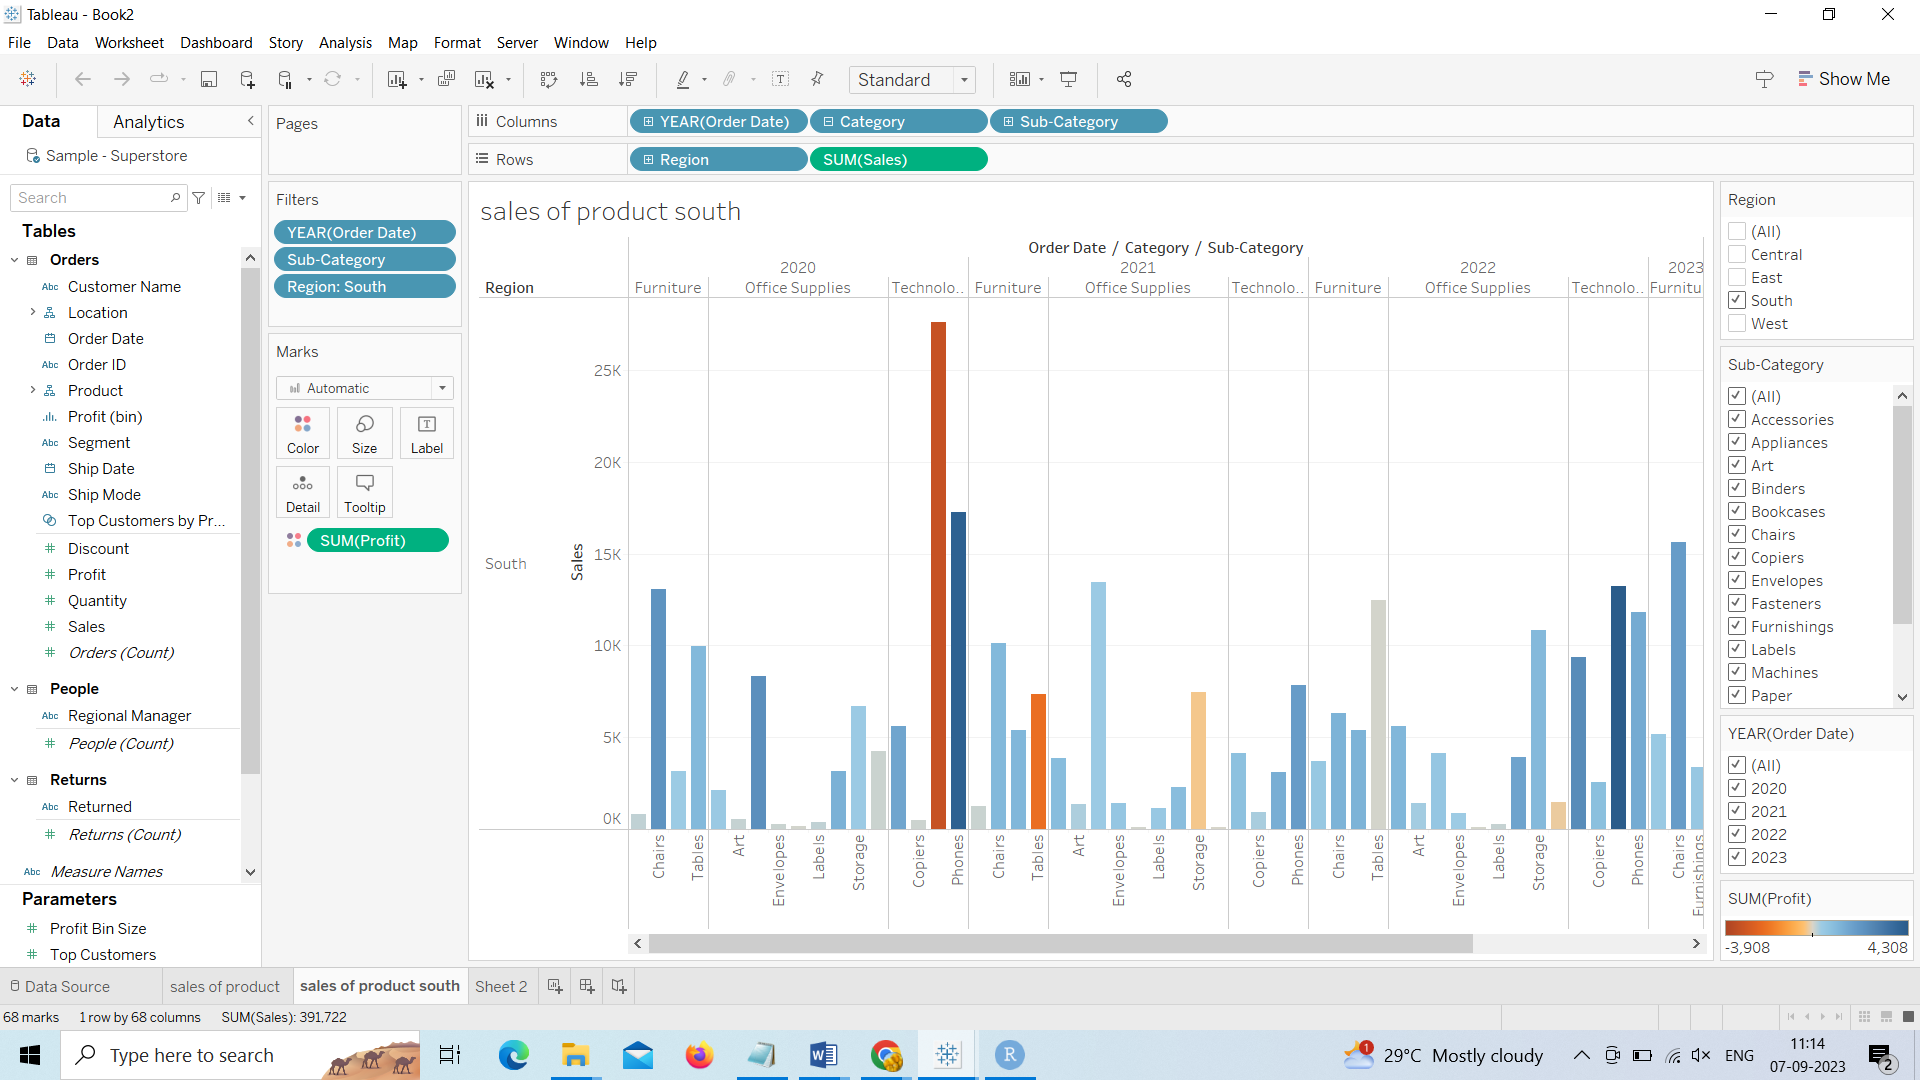
\includegraphics{tableau.png} \#\# Google Colab

\emph{What is the URL of your Google Colab notebook?}

\begin{verbatim}
 https://colab.research.google.com/drive/1edLxzvehDprqhVh4wwvvL_-toNlxdg-e?usp=sharing
\end{verbatim}

\textbf{Python/Seaborn}

\emph{Insert the first penguin chart here}

\begin{figure}
\centering
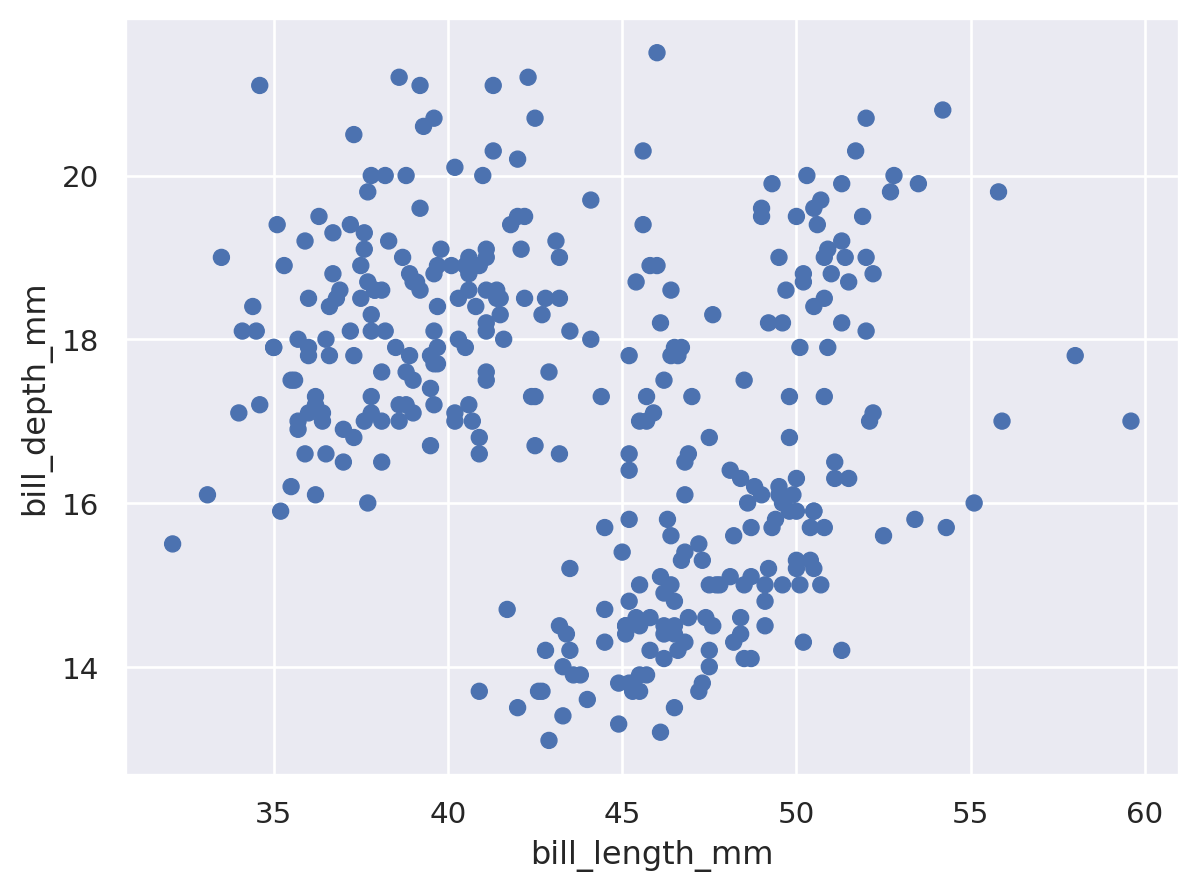
\includegraphics{1.png}
\caption{1}
\end{figure}

\emph{Describe what the figure is showing.}

\begin{verbatim}
 In the above image the graph presents the information about bill_length_mm and bill_depth_mm in x and y axes, where bill_length_mm with range 35 to 60 and bill_depth_mm with range 14 to 20
\end{verbatim}

\emph{Insert the second penguin chart here}

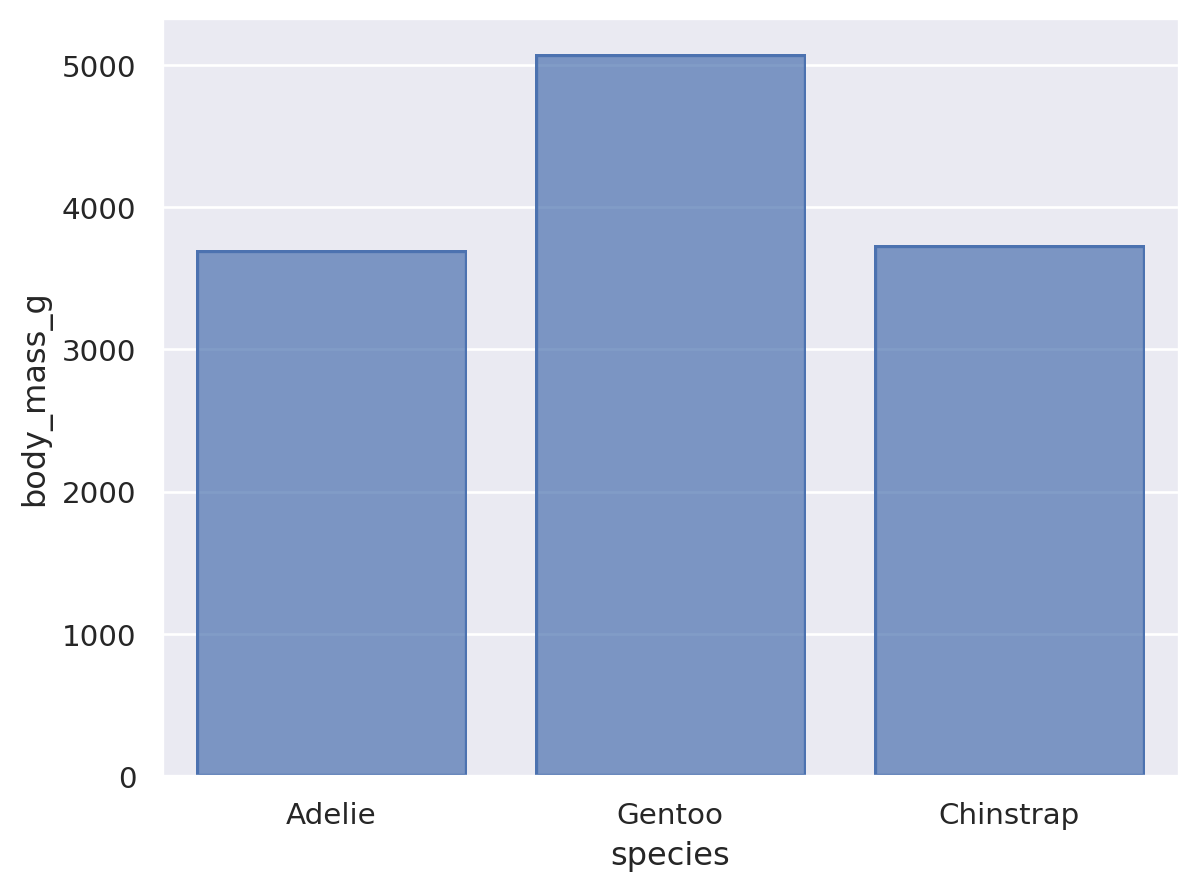
\includegraphics{2.png} \emph{Describe what the figure is showing.} From
the above Bar graph by comparison we can say that the body mass in
Gentoo is approx. 5000 which is greater than Adelie and Chinstrap, where
Adelie and Chinstrap lies in between 3000 -- 4000. \emph{What happened
when you removed the outer parentheses from the code? Why?}

\hypertarget{observable-and-vega-lite}{%
\subsection{Observable and Vega-Lite}\label{observable-and-vega-lite}}

\emph{What happens when you replace \texttt{markCircle()} with
\texttt{markSquare()}?}

\begin{verbatim}
markCircle() is used to mark or highlight something as a circle shape where as markSquare() is used to mark or highlight something as a square shape.
\end{verbatim}

\emph{What happens when you replace \texttt{markCircle()} with
\texttt{markPoint()}?}

\begin{verbatim}
markCircle() respresents the highlighted part in a circle, whereas markPoint() represents the highlighted part in small circles and can be used for custome representation also.
\end{verbatim}

\emph{What change do you need to make to swap the x and y axes on the
scatterplot?}

\begin{verbatim}
vl.x().fieldQ("Horsepower") vl.y().fieldQ("Miles_per_Gallon") should be replaced by vl.y().fieldQ("Horsepower") vl.x().fieldQ("Miles_per_Gallon") to swap the x and y axes .
\end{verbatim}

\emph{Insert the bar chart image here}

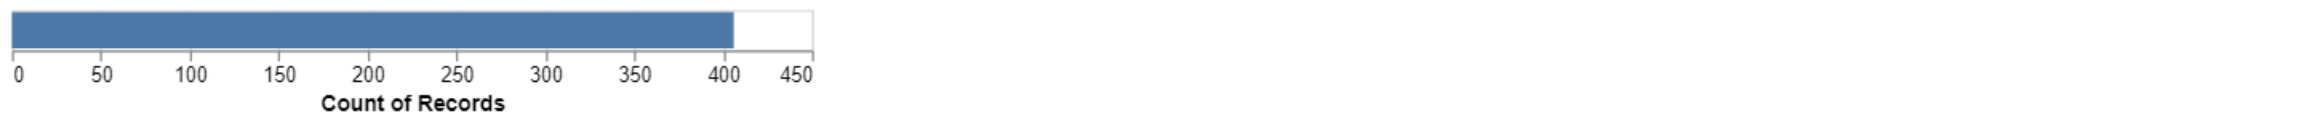
\includegraphics{vega-chart.png} \emph{Why do you think this chart is
the result of this code change?} Because of the change in the code
y-axis is missing which is vl.y().fieldN(``Origin''), we can only see
this x-axis which shows the record count. \#\# References

\emph{Every report must list the references (including the URL) that you
consulted while completing the assignment. Replace the items below with
the references you consulted}

\begin{itemize}
\tightlist
\item
  Reference 1, \url{https://chat.openai.com/}
\item
  Reference 2,
  \url{https://vega.github.io/vega-lite/tutorials/getting_started.html}
\end{itemize}

\end{document}
